\newpage
\section{Decision Trees}
\label{sec:decision-trees}

This section evaluates single decision-tree classifiers for churn prediction. Decision trees are useful at this stage because they introduce nonlinear, rule-based classification without yet using ensembles. A fitted tree partitions the transformed feature space into regions, assigns each region a local churn proportion, and uses that local proportion both for hard classification and for ranking customers by churn risk.

The same development discipline is used as in the previous modelling sections. The held-out test set is not used. All reported results are based on stratified cross-validation inside the training set, using out-of-fold predictions where possible. The comparisons in this section are therefore development-stage comparisons of decision-tree variants. They identify a representative single-tree candidate within the tried configurations, but they are not final test-set performance claims.

\subsection{Recursive partitioning}

Let the training data be
\[
\mathcal{D}_{\mathrm{train}}
=
\{(x_i,y_i)\}_{i=1}^{n},
\]
where \(x_i\) is the transformed customer feature vector and \(y_i\in\{0,1\}\) is the churn label. A decision tree recursively splits the feature space into smaller regions. Each internal node applies a rule of the form
\[
x_j \leq s,
\]
where \(x_j\) is one feature and \(s\) is a split value. For one-hot encoded categorical indicators, these split rules often test whether a category indicator is zero or one.

After the recursive splitting process, each terminal node or leaf contains a subset of training observations. For a leaf \(R_m\), the estimated churn probability is the local class proportion:
\[
\widehat{p}_m
=
\frac{1}{|R_m|}
\sum_{i:x_i\in R_m} y_i.
\]
For a new customer \(x\), the fitted tree sends \(x\) to one leaf and predicts
\[
\widehat{p}(Y=1\mid X=x)=\widehat{p}_m.
\]
The default hard prediction at threshold \(0.5\) is
\[
\widehat{y}
=
\mathbb{1}\{\widehat{p}(Y=1\mid X=x)\geq 0.5\}.
\]
Thus, a classification tree can be interpreted as a collection of local empirical churn-rate rules.

\subsection{Split selection and impurity}

Tree construction is greedy. At a node, the algorithm evaluates candidate feature-threshold splits and chooses the split that most improves class purity. It does not search globally over all possible trees, because the number of possible tree structures is too large.

For binary classification, one common impurity measure is the Gini impurity. If a node has churn proportion \(p\), its Gini impurity is
\[
G(p)
=
1-p^2-(1-p)^2
=
2p(1-p).
\]
The impurity is zero when the node is pure, meaning \(p=0\) or \(p=1\). It is largest when the node is evenly mixed, meaning \(p=0.5\).

For a candidate split that divides a parent node \(R\) into left and right children \(R_L\) and \(R_R\), the weighted child impurity is
\[
G_{\mathrm{children}}
=
\frac{|R_L|}{|R|}G(R_L)
+
\frac{|R_R|}{|R|}G(R_R).
\]
The split improvement is
\[
\Delta G
=
G(R)-G_{\mathrm{children}}.
\]
The greedy algorithm chooses the candidate split with the largest impurity reduction. Entropy and information gain follow the same logic, but use
\[
H(p)
=
-p\log(p)-(1-p)\log(1-p)
\]
instead of Gini impurity.

\subsection{Ranking with decision trees}

Although decision trees are often described as rule-based classifiers, they also produce scores. The score for a customer is the estimated churn proportion in the leaf that the customer reaches. Therefore, decision trees rank customers by leaf churn rate.

This ranking has a specific structure. All customers in the same leaf receive exactly the same score, so the ranking is stepwise and can contain many ties. A shallow or strongly pruned tree has fewer leaves and therefore fewer possible score levels. This makes its ranking coarse but often more stable. A deeper tree has more leaves and more possible score levels, but the estimated leaf probabilities can be noisy when leaves contain few observations.

This matters for ROC-AUC and precision-recall analysis. Trees are trained by local impurity reduction, not by directly optimizing ROC-AUC or PR-AUC. Ranking quality must therefore be evaluated explicitly from out-of-fold predicted probabilities.

\subsection{Regularization and pruning}

Unrestricted decision trees can overfit. A deep tree can keep splitting until leaves become very small, fitting local noise and idiosyncratic training patterns. This lowers training impurity but can harm validation performance.

This section evaluates two forms of tree regularization. The first is pre-pruning, where tree growth is restricted during fitting through hyperparameters such as
\[
\texttt{max\_depth},\qquad
\texttt{min\_samples\_split},\qquad
\texttt{min\_samples\_leaf}.
\]
The second is cost-complexity pruning, controlled in scikit-learn by \(\texttt{ccp\_alpha}\). Cost-complexity pruning grows a large tree and then selects a smaller subtree by penalizing complexity. Conceptually, the pruning criterion has the form
\[
\text{training impurity}
+
\alpha \times \text{tree complexity},
\]
where larger \(\alpha\) favours smaller trees.

The pruning parameter is a hyperparameter like \(\texttt{max\_depth}\) or \(\texttt{min\_samples\_leaf}\). In this section it is selected with cross-validation inside the training set. This is appropriate for development-stage model selection. However, if a separate validation set were reserved for higher-level model-family comparison, that same validation set should not also be used to choose the pruning level. A stricter estimate of the full tune-and-select procedure would require nested validation. This section does not claim to provide such a final unbiased estimate; final testing remains deferred.

\subsection{Experimental design}

Four decision-tree variants are evaluated:

\begin{itemize}[leftmargin=*]
    \item \textbf{Decision stump}: a depth-one tree.
    \item \textbf{Default decision tree}: an unrestricted baseline tree.
    \item \textbf{Pre-pruned tree grid}: a grid over \(\texttt{criterion}\), \(\texttt{max\_depth}\), \(\texttt{min\_samples\_split}\), and \(\texttt{min\_samples\_leaf}\).
    \item \textbf{Cost-complexity-pruned tree grid}: a grid over candidate \(\texttt{ccp\_alpha}\) values.
\end{itemize}

The representative decision tree is selected by cross-validated PR-AUC, with balanced accuracy and \(F_1\) used as secondary criteria. PR-AUC remains the primary criterion because churn is the minority class and positive-class retrieval is central to the project.

\subsection{Pre-pruning results}

Figure~\ref{fig:decision-tree-prepruned-pr-auc} shows the pre-pruning grid from the perspective of PR-AUC. Very shallow trees underfit the ranking problem, while moderately deep trees perform better. The best PR-AUC occurs at depth 6 with \(\texttt{min\_samples\_leaf}=10\). The unrestricted-depth setting performs worse, especially when \(\texttt{min\_samples\_leaf}=1\), which is consistent with overfitting.

\begin{figure}[H]
\centering
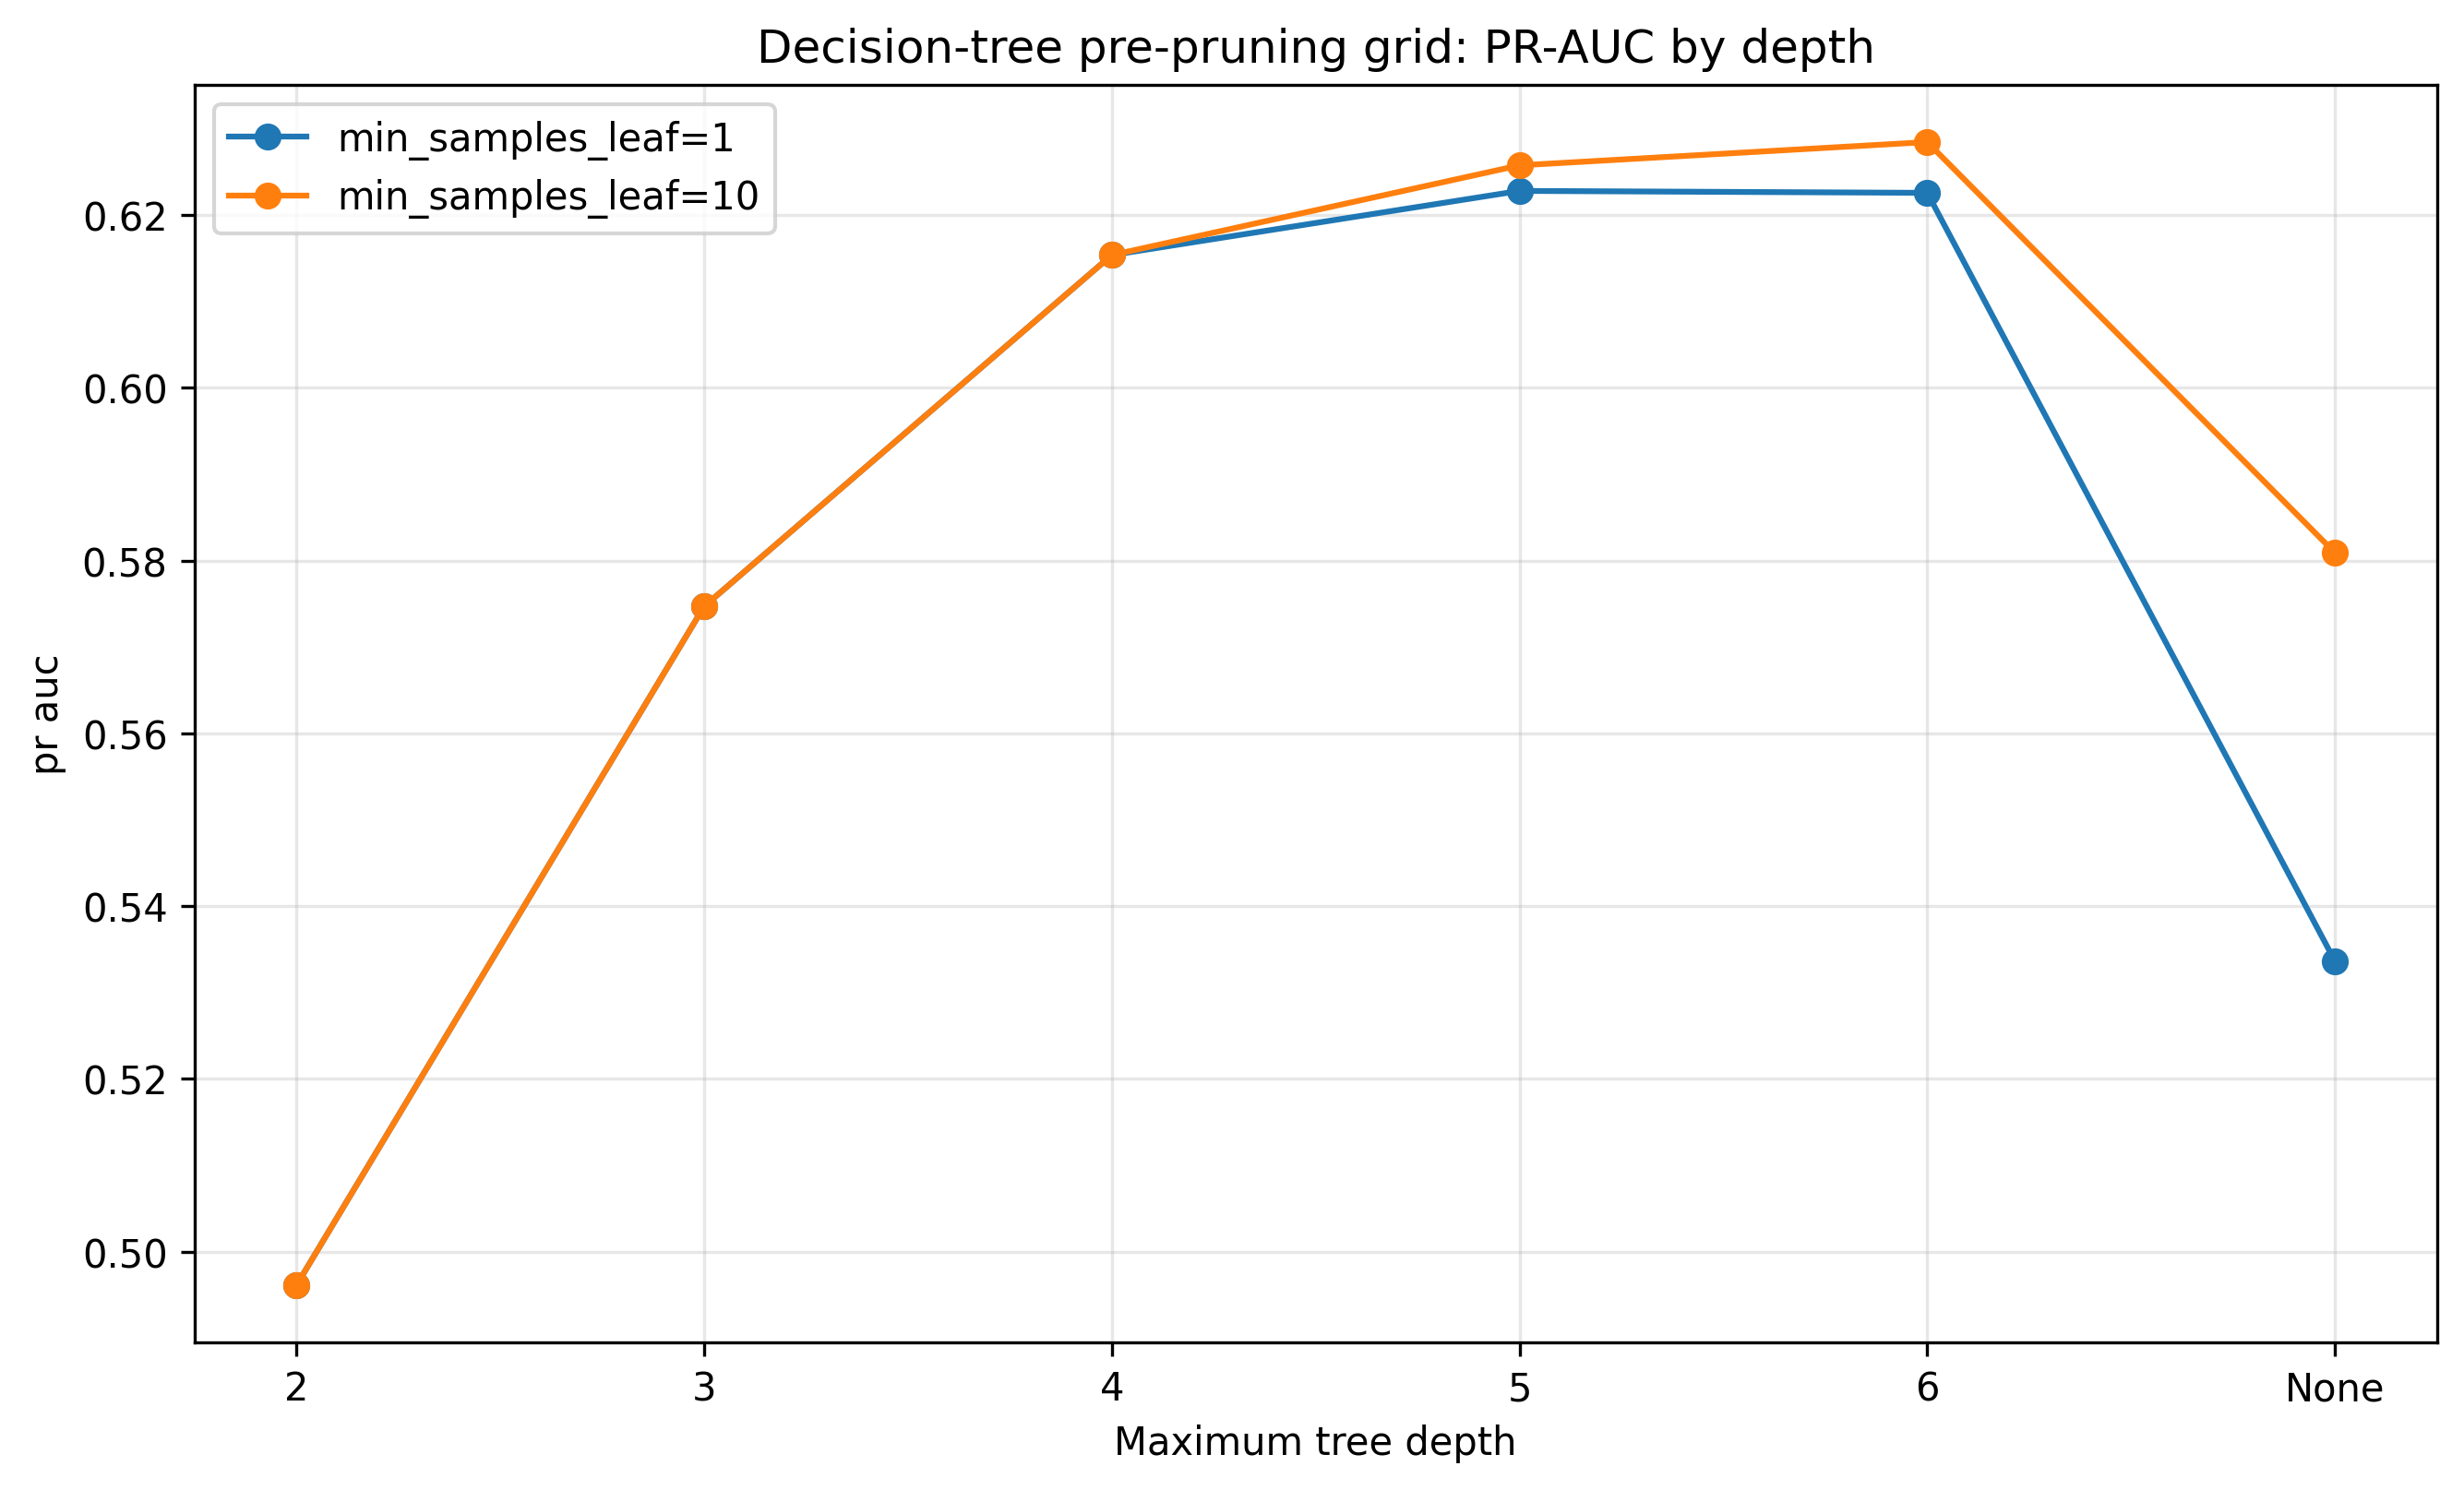
\includegraphics[width=0.88\textwidth]{../figures/decision_tree_prepruned_pr_auc_by_depth.png}
\caption{Decision-tree pre-pruning grid: PR-AUC by maximum depth}
\label{fig:decision-tree-prepruned-pr-auc}
\end{figure}

Figure~\ref{fig:decision-tree-prepruned-balanced-accuracy} shows the same grid using balanced accuracy. The depth-two tree has high balanced accuracy but weak PR-AUC, showing that a good default-threshold class split is not the same as strong ranking performance. The depth-five and depth-six trees provide stronger ranking performance while keeping the tree sufficiently regularized.

\begin{figure}[H]
\centering
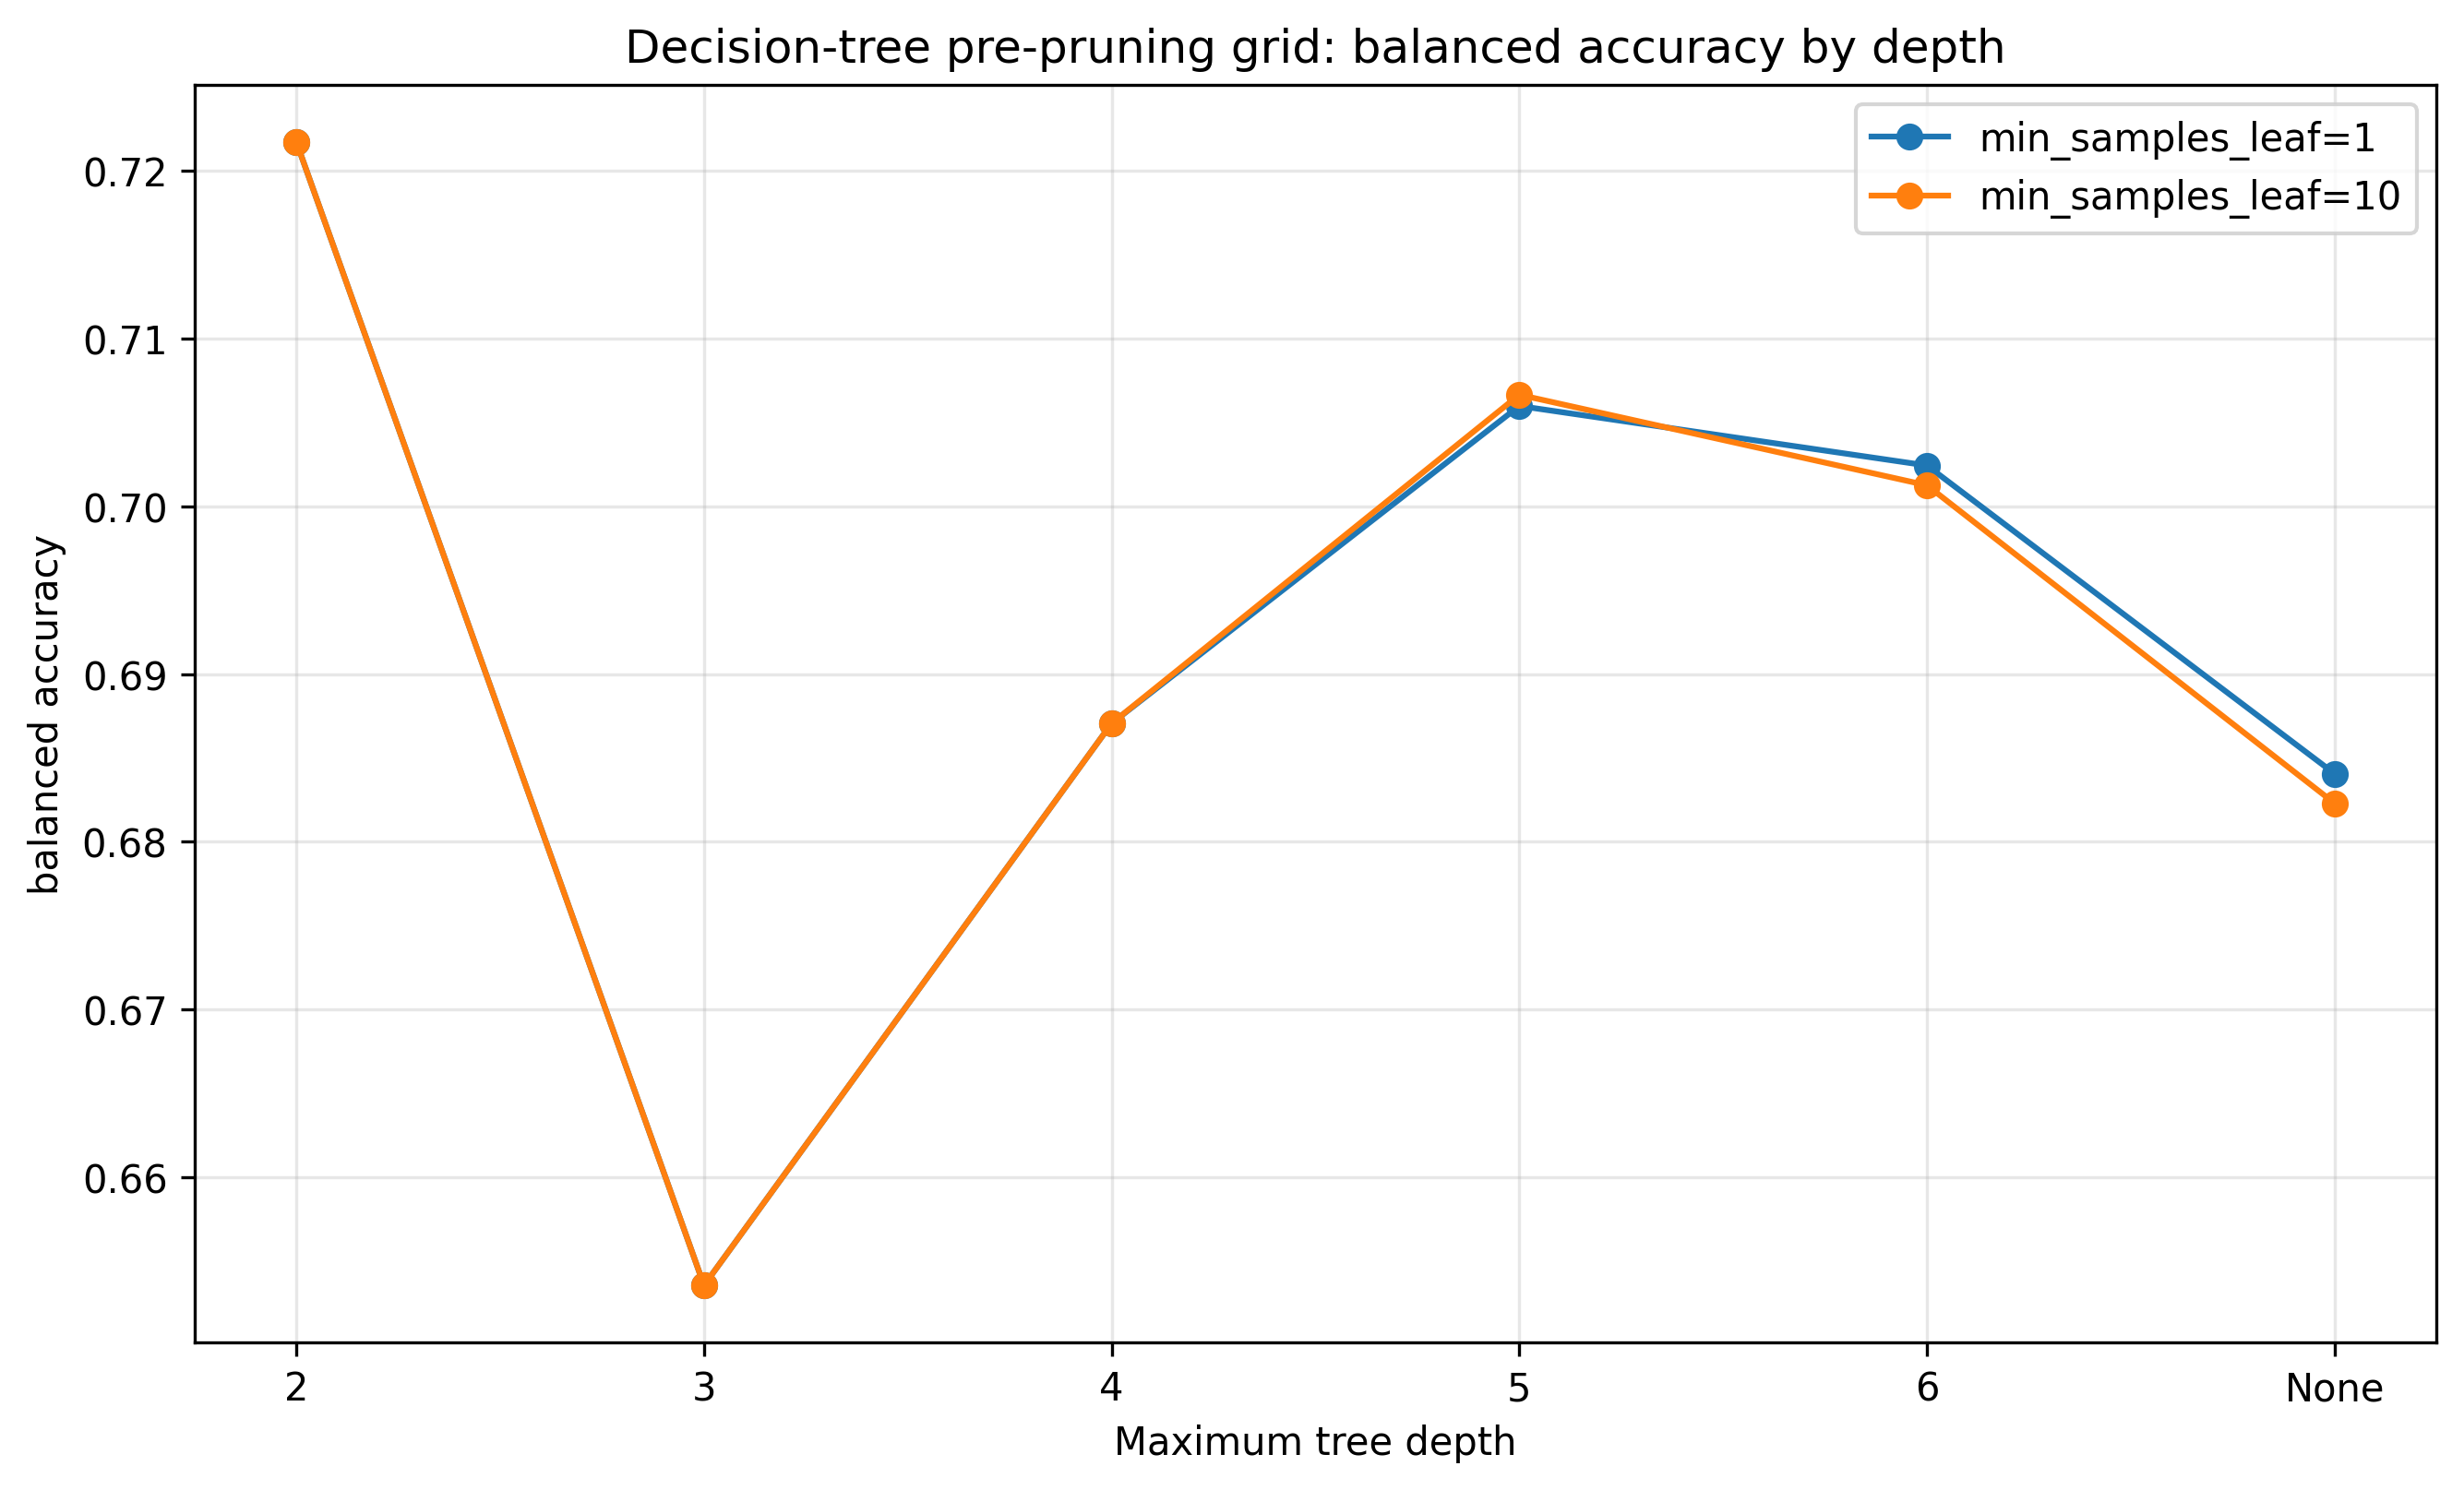
\includegraphics[width=0.88\textwidth]{../figures/decision_tree_prepruned_balanced_accuracy_by_depth.png}
\caption{Decision-tree pre-pruning grid: balanced accuracy by maximum depth}
\label{fig:decision-tree-prepruned-balanced-accuracy}
\end{figure}

\subsection{Cost-complexity pruning results}

Figure~\ref{fig:decision-tree-ccp-alpha} shows the cost-complexity pruning grid. The unpruned tree has weak PR-AUC because it overfits. As \(\texttt{ccp\_alpha}\) increases, the tree becomes smaller and the ranking metrics improve substantially. The best cost-complexity-pruned tree reaches PR-AUC approximately \(0.615\), which is much better than the default unrestricted tree but still below the best pre-pruned tree.

\begin{figure}[H]
\centering
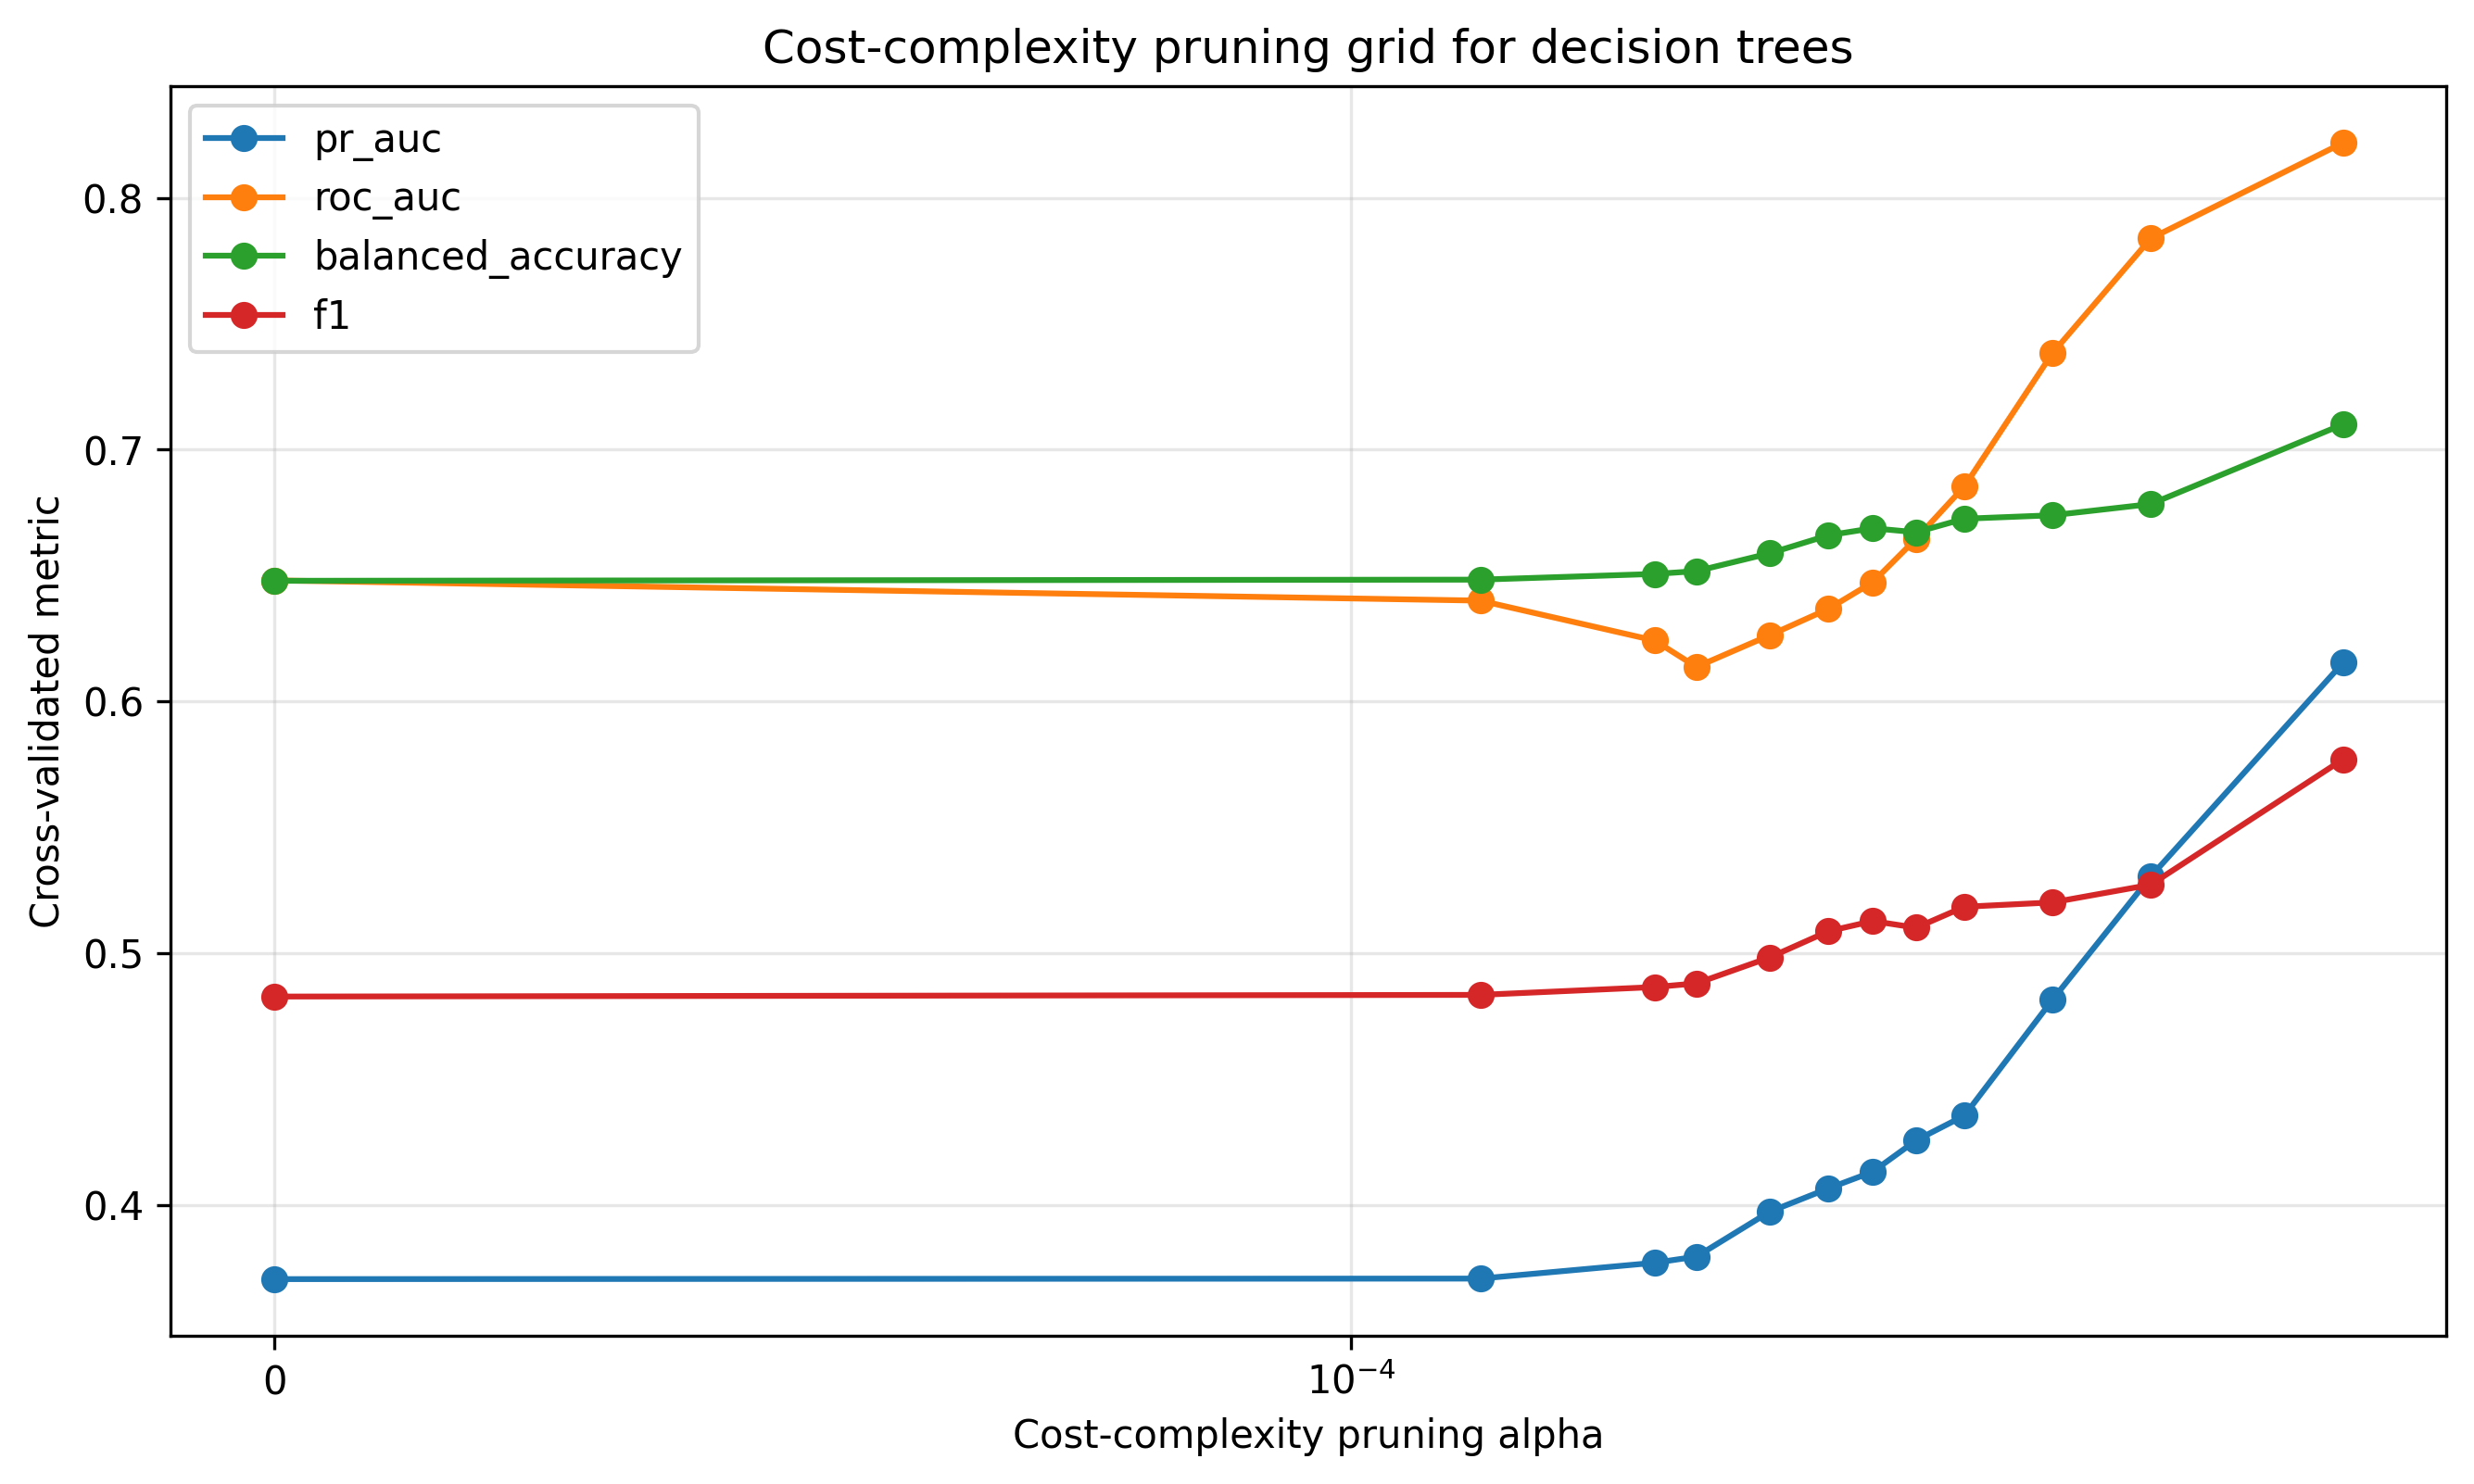
\includegraphics[width=0.88\textwidth]{../figures/decision_tree_ccp_alpha_metrics.png}
\caption{Cost-complexity pruning metrics for decision trees}
\label{fig:decision-tree-ccp-alpha}
\end{figure}

The pruning result is useful because it demonstrates the central decision-tree bias-variance tradeoff. A larger tree can fit training irregularities, but a smaller pruned tree can generalize better. In this dataset, however, direct pre-pruning with a moderate maximum depth and minimum leaf size gives the strongest single-tree ranking result.

\subsection{Model comparison}

Table~\ref{tab:decision-tree-model-comparison} compares the main decision-tree variants. The selected model is a Gini tree with \(\texttt{max\_depth}=6\), \(\texttt{min\_samples\_split}=25\), \(\texttt{min\_samples\_leaf}=10\), and \(\texttt{ccp\_alpha}=0\). It has PR-AUC approximately \(0.628\) and ROC-AUC approximately \(0.824\). It improves sharply over the default unrestricted tree, whose PR-AUC is only approximately \(0.371\).

\begin{table}[H]
\centering
\small
\resizebox{\textwidth}{!}{
\begin{tabular}{lrrrrrrrr}
\toprule
Model & Accuracy & Bal. Acc. & Precision & Recall & Specificity & \(F_1\) & ROC-AUC & PR-AUC \\
\midrule
Selected pre-pruned tree & 0.789 & 0.701 & 0.624 & 0.514 & 0.888 & 0.564 & 0.824 & 0.628 \\
Best cost-complexity-pruned tree & 0.790 & 0.710 & 0.620 & 0.540 & 0.880 & 0.577 & 0.822 & 0.615 \\
Decision stump & 0.735 & 0.500 & 0.000 & 0.000 & 1.000 & 0.000 & 0.726 & 0.413 \\
Default unrestricted tree & 0.725 & 0.648 & 0.482 & 0.484 & 0.812 & 0.483 & 0.648 & 0.371 \\
\bottomrule
\end{tabular}
}
\caption{Cross-validated decision-tree model comparison on the training set}
\label{tab:decision-tree-model-comparison}
\end{table}

The corresponding positive-first confusion-matrix counts are shown in Table~\ref{tab:decision-tree-confusion}. At the default threshold, the selected pre-pruned tree detects \(769\) of the \(1495\) churners and misses \(726\). It flags \(463\) non-churners as churn risks and correctly classifies \(3676\) non-churners.

\begin{table}[H]
\centering
\small
\begin{tabular}{lrrrr}
\toprule
Model & TP & FN & FP & TN \\
\midrule
Selected pre-pruned tree & 769 & 726 & 463 & 3676 \\
Best cost-complexity-pruned tree & 807 & 688 & 495 & 3644 \\
Decision stump & 0 & 1495 & 0 & 4139 \\
Default unrestricted tree & 723 & 772 & 777 & 3362 \\
\bottomrule
\end{tabular}
\caption{Positive-first confusion-matrix counts for decision-tree models}
\label{tab:decision-tree-confusion}
\end{table}

The decision stump has ordinary accuracy equal to the no-churn majority baseline and predicts no churn at the default threshold. Nevertheless, its ROC-AUC is above \(0.7\), because the stump still assigns different leaf probabilities and therefore contains some ranking information. This illustrates why hard classification metrics and ranking metrics answer different questions.

Compared with previous model families, the selected tree is useful but not dominant. It is much better than the default unrestricted tree and stronger than Naive Bayes by PR-AUC, but it remains below logistic regression from Section~\ref{sec:linear-classification-and-logistic-regression}. Its PR-AUC is close to selected k-nearest neighbours from Section~\ref{sec:knn}. This supports continuing to tree ensembles later: a single tree captures meaningful nonlinear churn structure, but its instability and coarse leaf-based scoring limit its standalone performance.

\subsection{Threshold behaviour}

Figure~\ref{fig:decision-tree-threshold-tradeoff} shows the threshold tradeoff for the selected tree. Lower thresholds increase recall but also create many more false positives. Higher thresholds improve precision and specificity, but recall falls.

\begin{figure}[H]
\centering
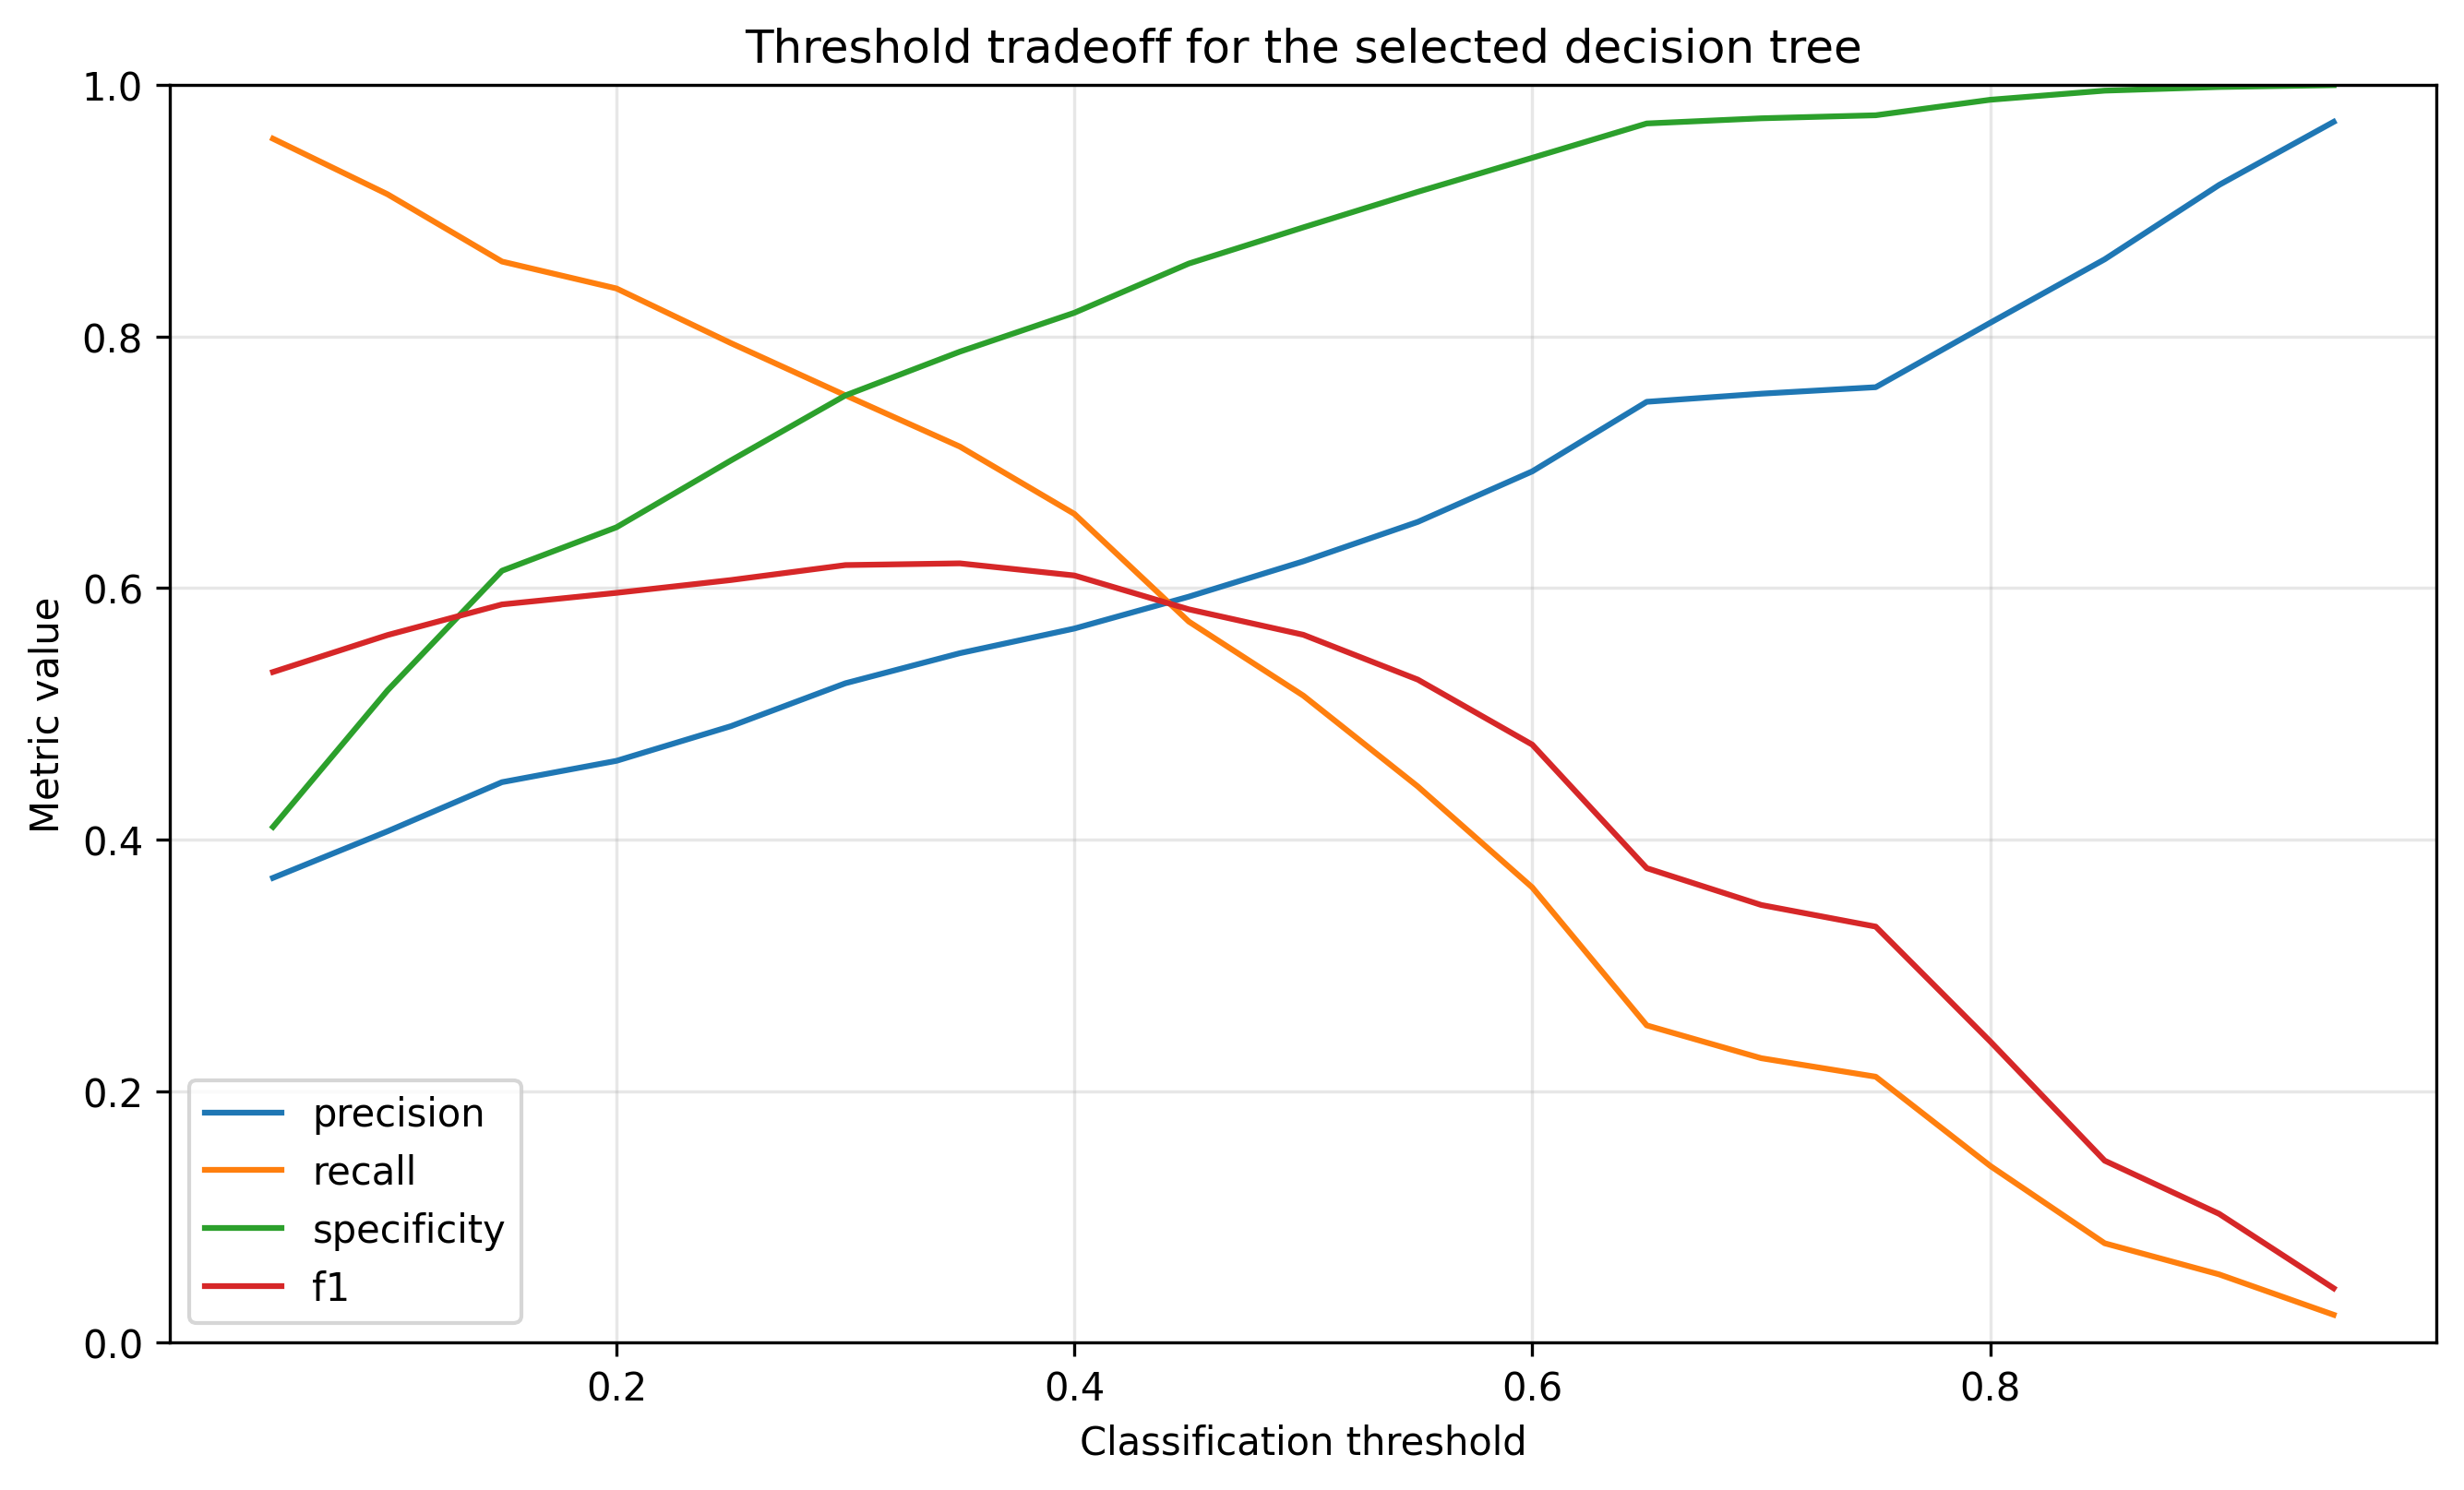
\includegraphics[width=0.88\textwidth]{../figures/decision_tree_threshold_tradeoff.png}
\caption{Threshold tradeoff for the selected decision tree}
\label{fig:decision-tree-threshold-tradeoff}
\end{figure}

At threshold \(0.30\), the selected tree has precision approximately \(0.524\), recall approximately \(0.753\), specificity approximately \(0.753\), and \(F_1\) approximately \(0.618\). At threshold \(0.35\), precision rises to approximately \(0.548\), recall is approximately \(0.712\), specificity is approximately \(0.788\), and \(F_1\) is approximately \(0.620\). At the default threshold \(0.50\), precision is approximately \(0.621\), recall falls to approximately \(0.514\), specificity rises to approximately \(0.887\), and \(F_1\) is approximately \(0.563\). This confirms again that the default threshold is not necessarily the best operating point for churn intervention.

\subsection{ROC and precision-recall curves}

Figure~\ref{fig:decision-tree-roc-curve} shows the ROC curve for the selected tree. The ROC-AUC is approximately \(0.824\), indicating useful ranking ability.

\begin{figure}[H]
\centering
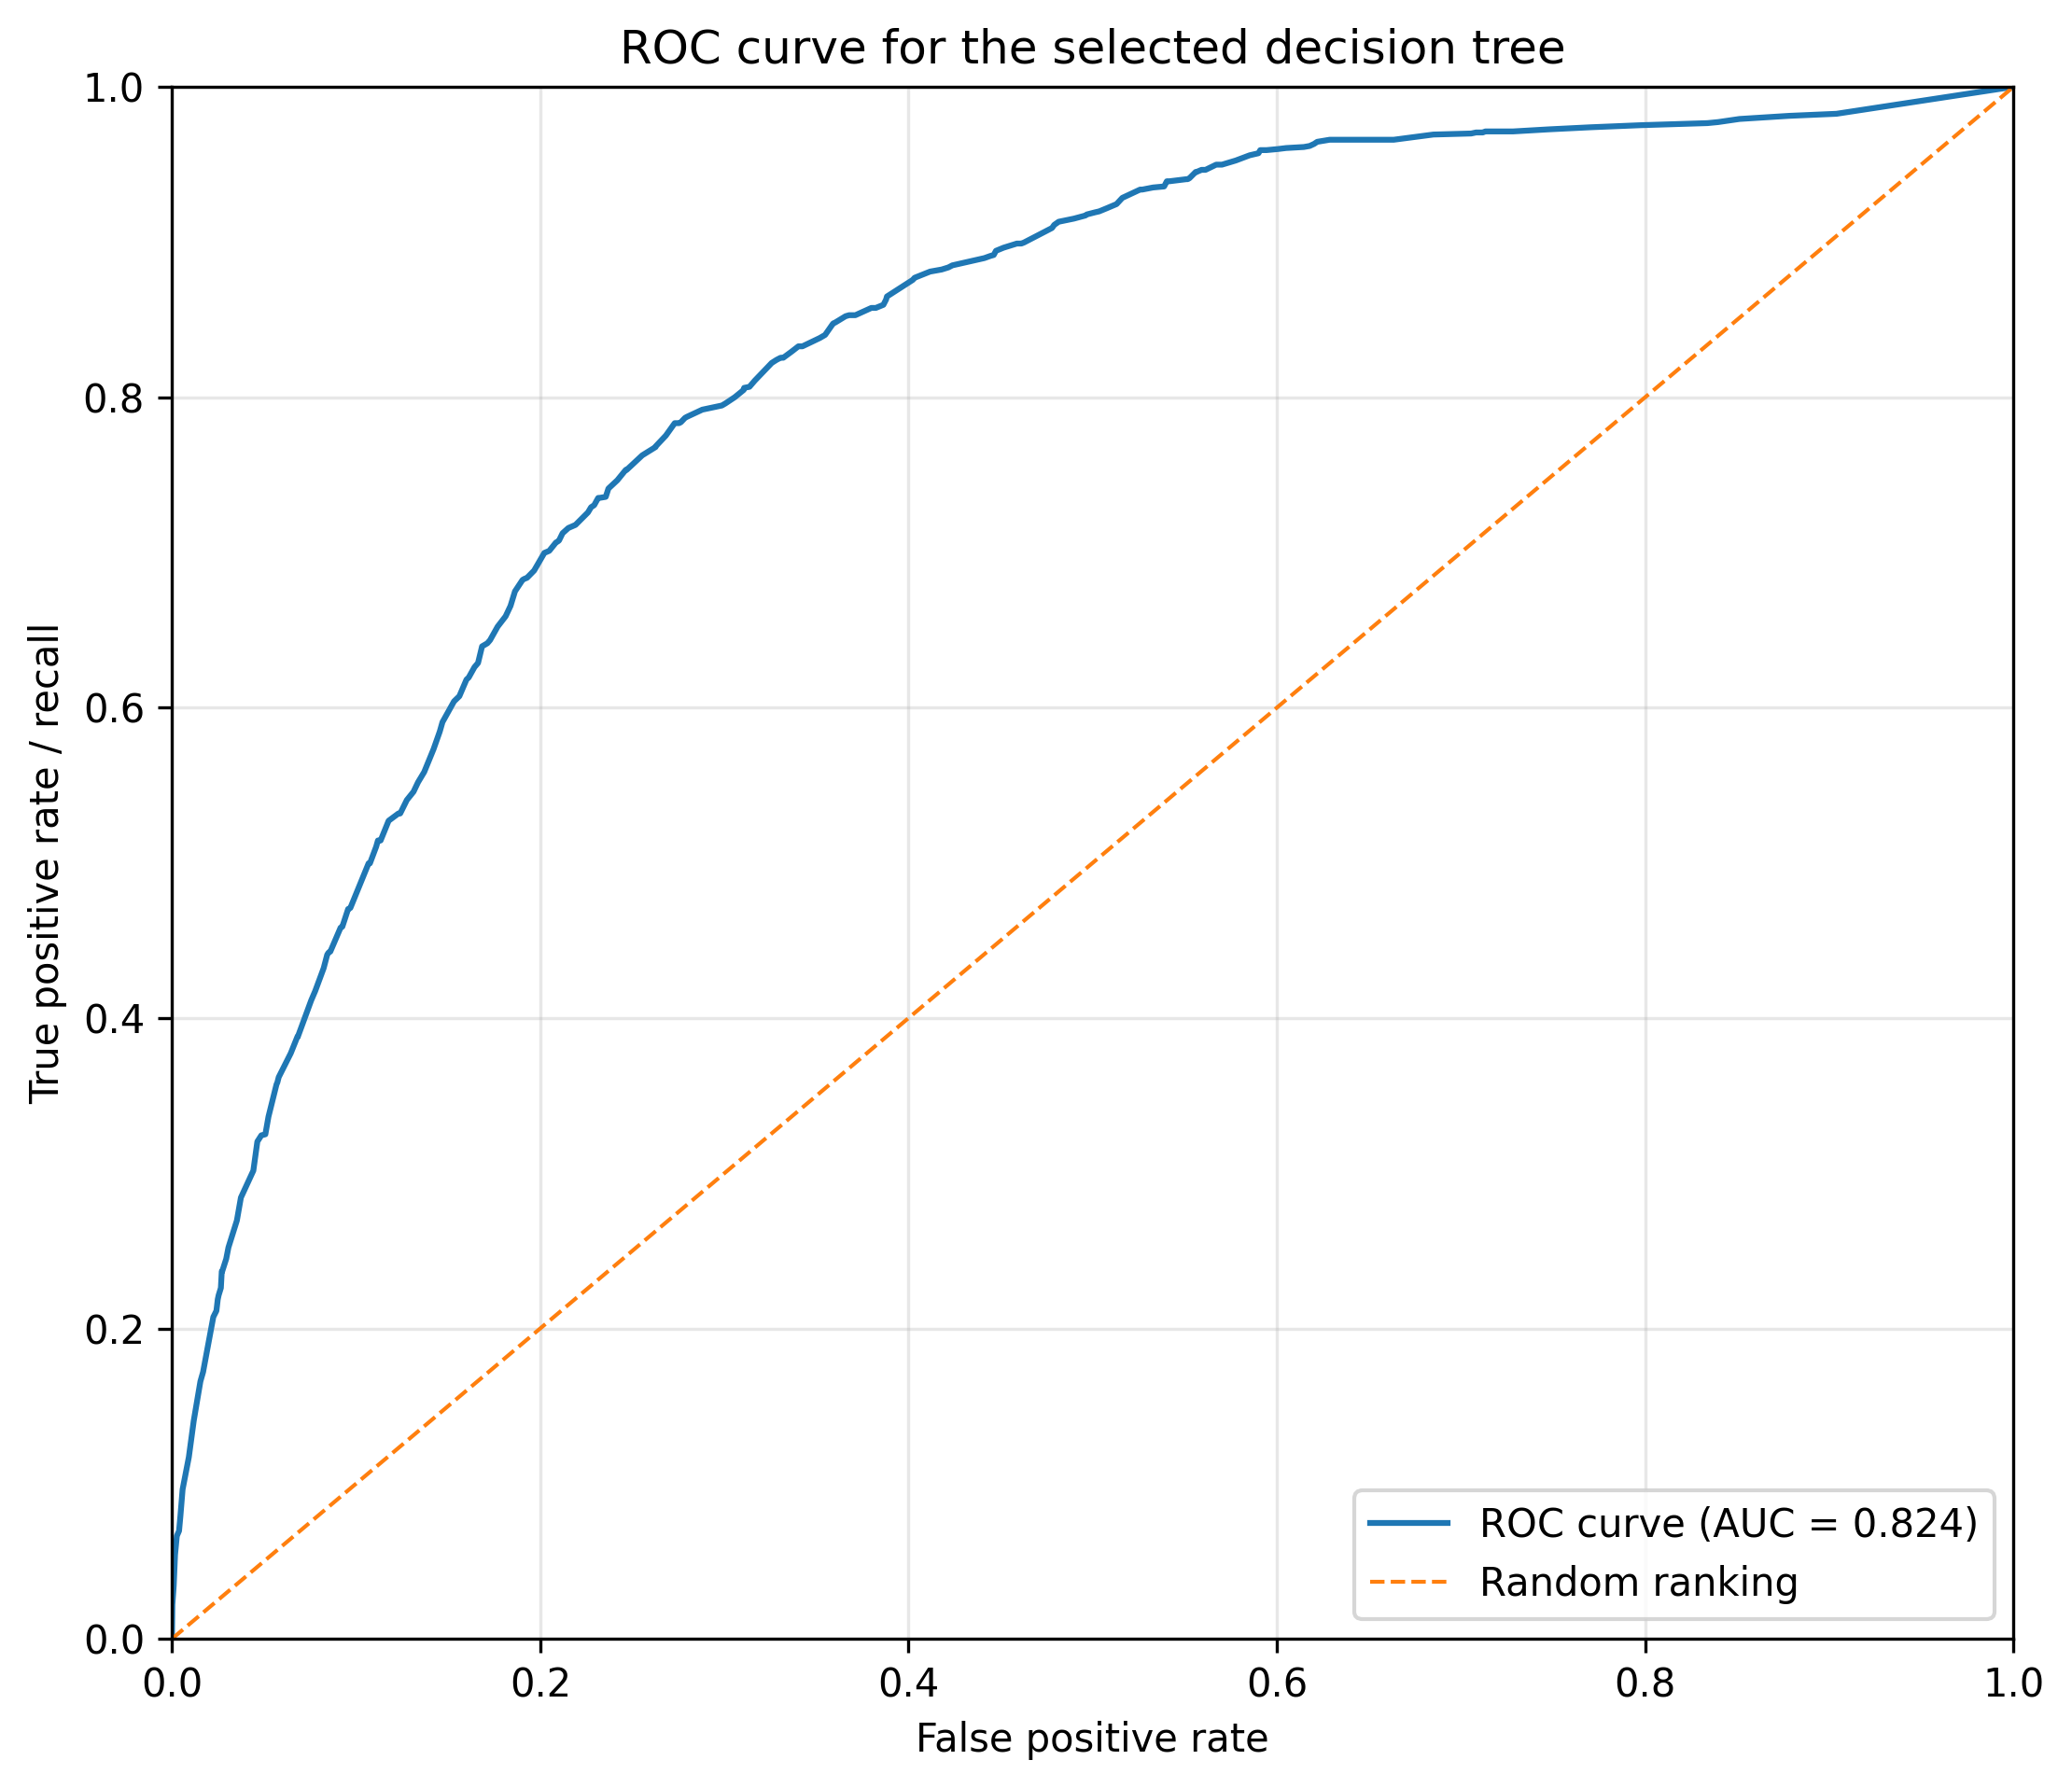
\includegraphics[width=0.72\textwidth]{../figures/decision_tree_roc_curve.png}
\caption{ROC curve for the selected decision tree}
\label{fig:decision-tree-roc-curve}
\end{figure}

Figure~\ref{fig:decision-tree-pr-curve} shows the precision-recall curve. The selected tree has PR-AUC around \(0.63\), well above the positive-rate baseline of approximately \(0.265\). This means that the tree ranks churners above non-churners much better than random ordering, even though its leaf-based probabilities produce a more stepwise ranking than smoother probabilistic models.

\begin{figure}[H]
\centering
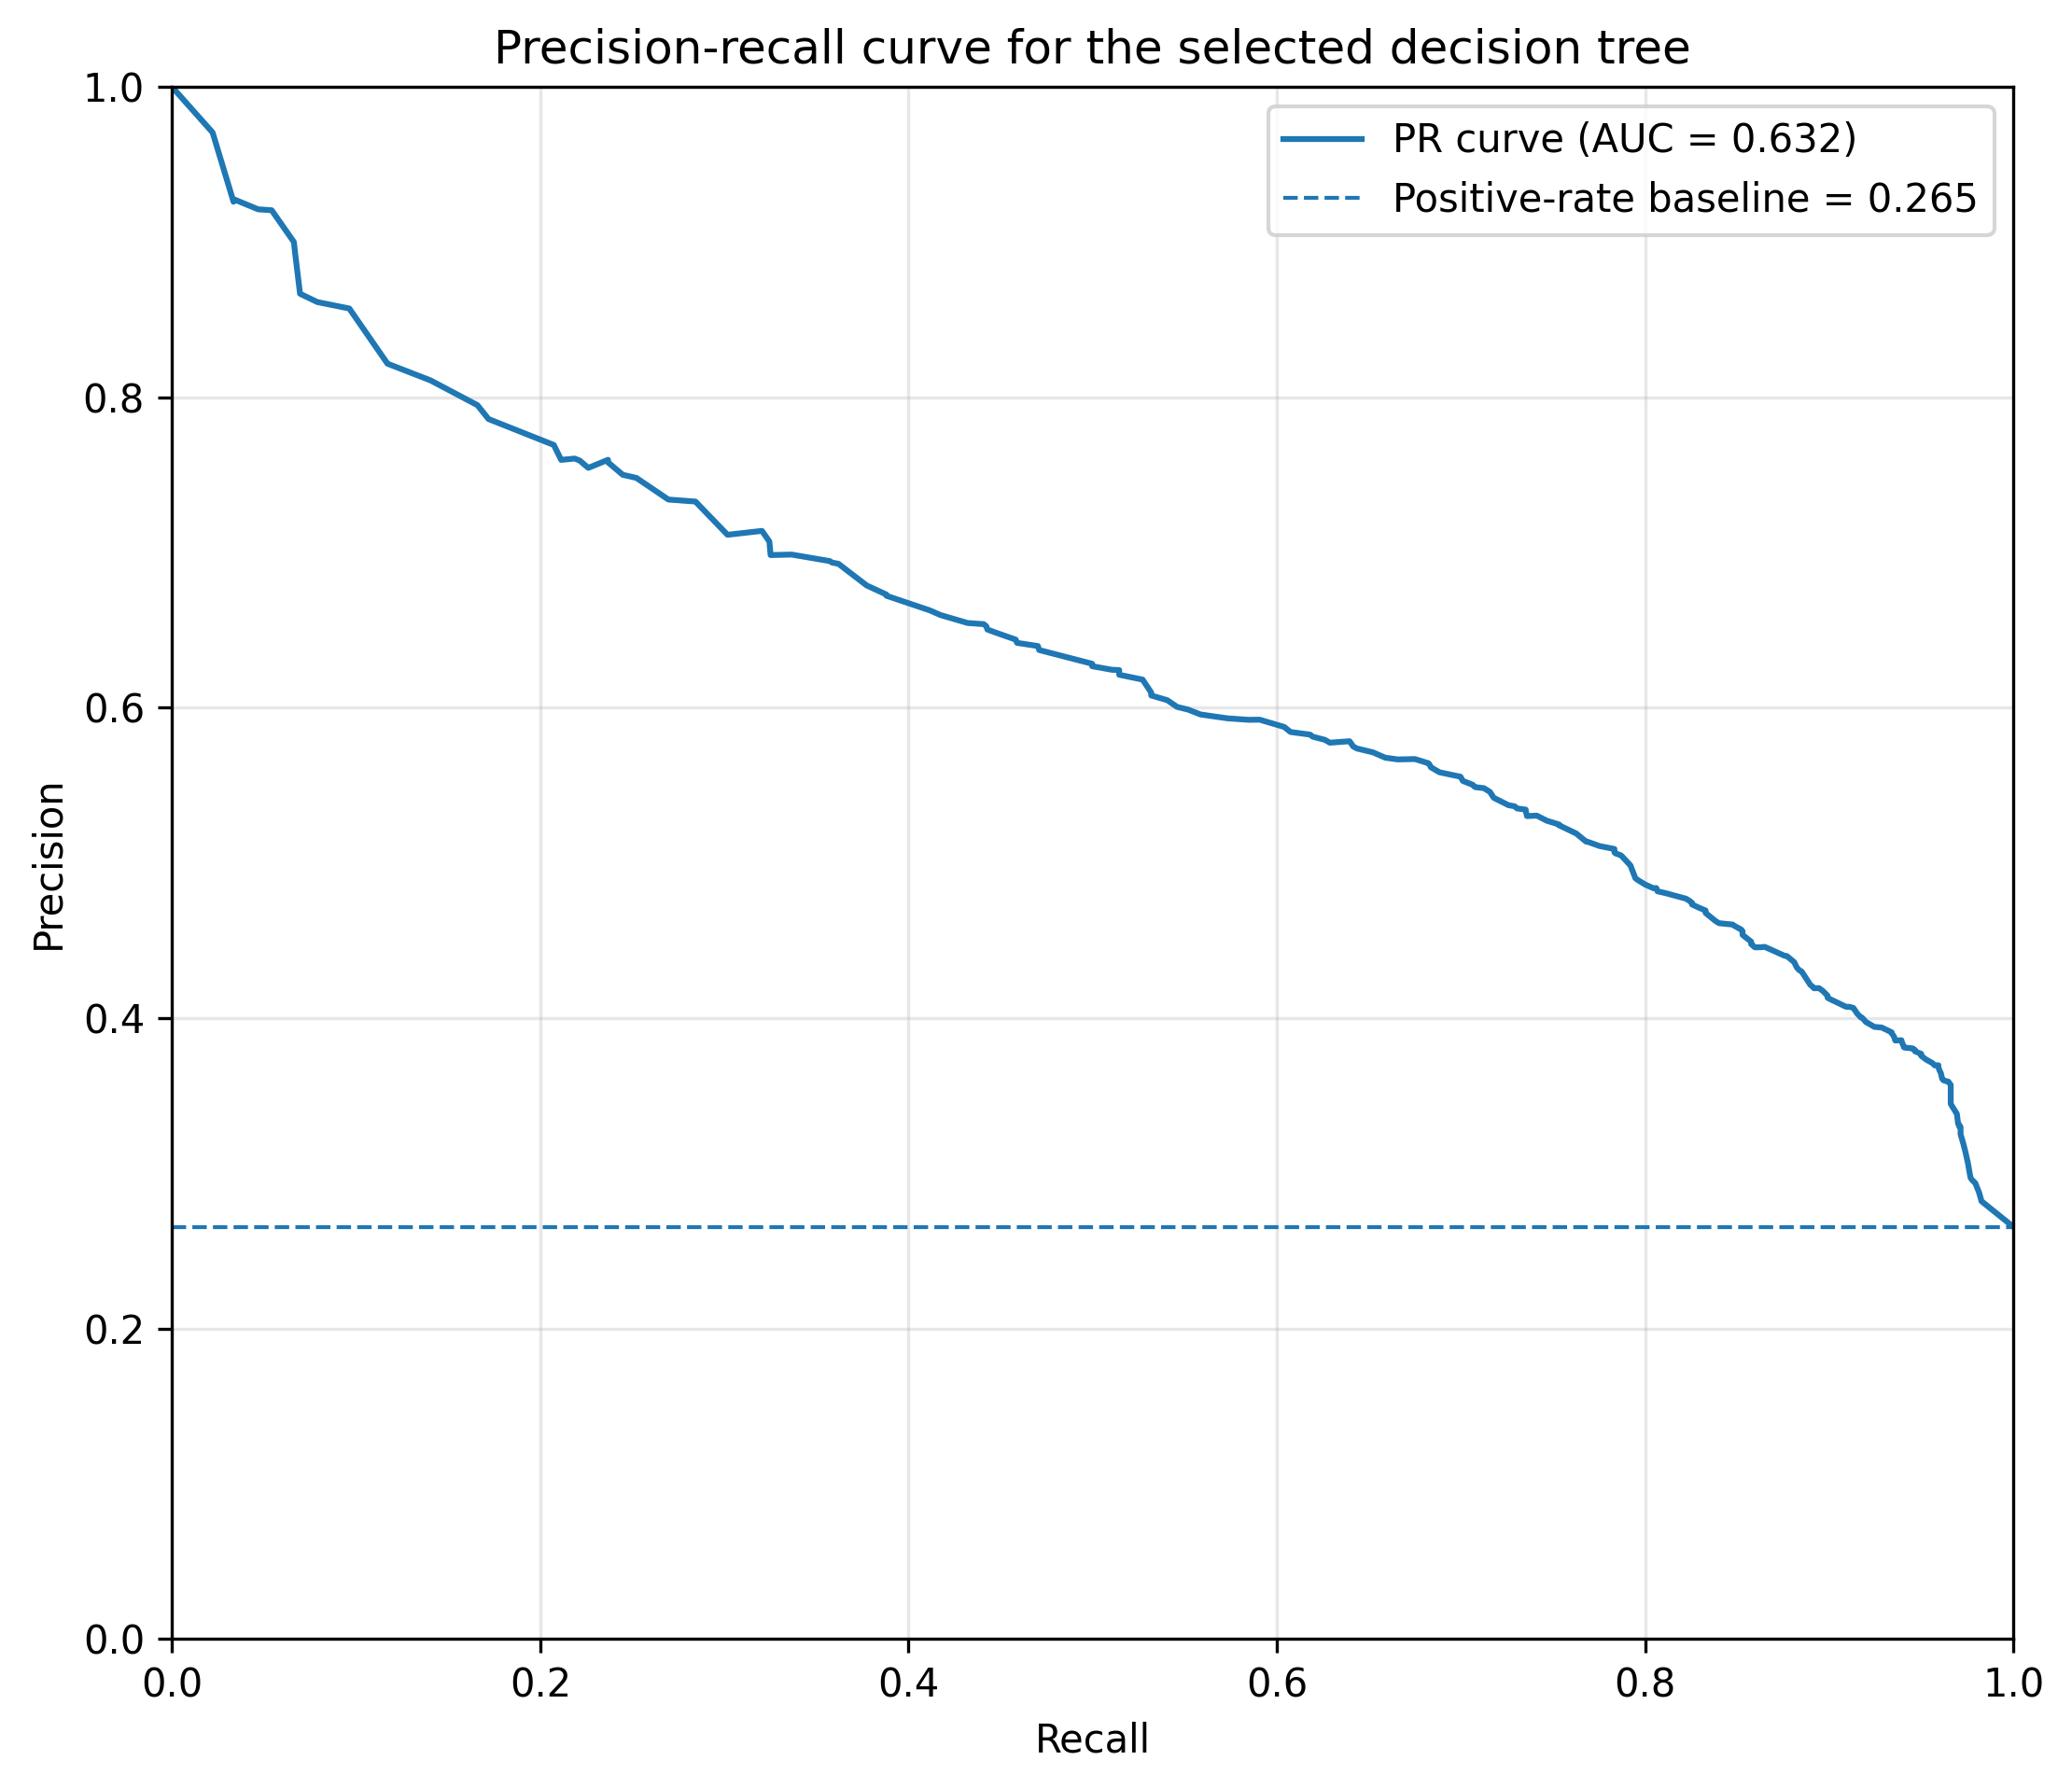
\includegraphics[width=0.72\textwidth]{../figures/decision_tree_precision_recall_curve.png}
\caption{Precision-recall curve for the selected decision tree}
\label{fig:decision-tree-pr-curve}
\end{figure}

\subsection{Interpretation of the selected tree}

The selected tree was refitted on the full training set only for interpretation. This refit is not used to estimate performance. Figure~\ref{fig:decision-tree-structure} shows the top levels of the fitted tree. The first split is on \texttt{Contract\_Month-to-month}, which is consistent with earlier EDA and logistic-regression results. Month-to-month contracts are a central churn-risk indicator.

\begin{figure}[H]
\centering
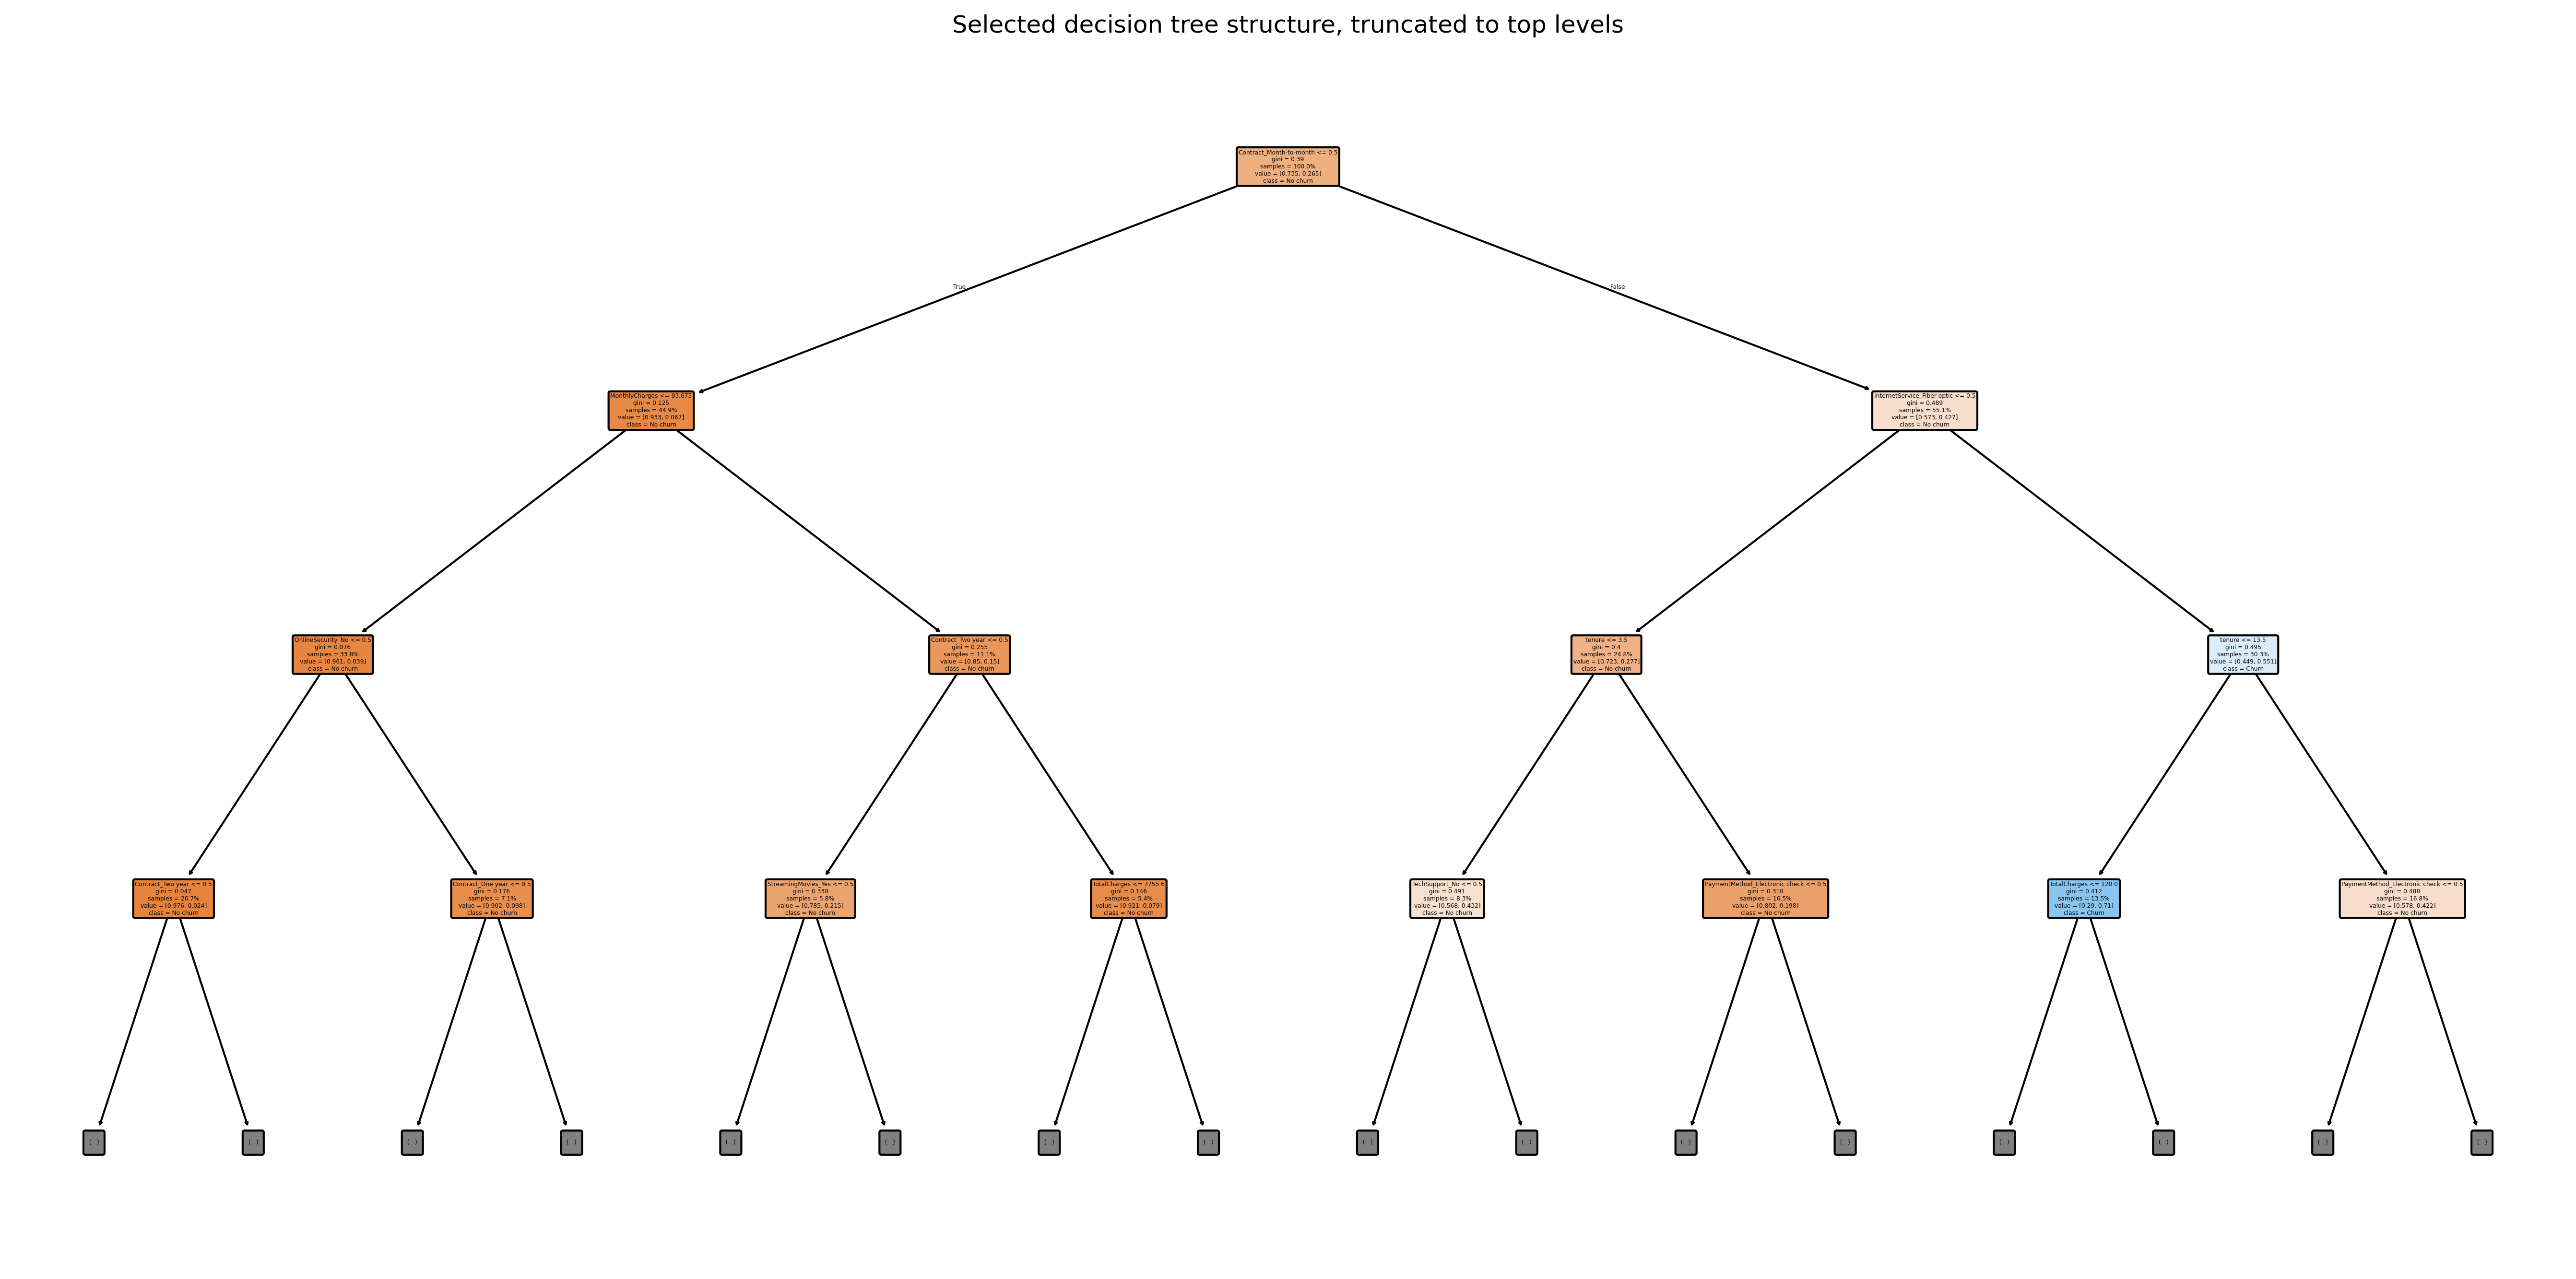
\includegraphics[width=\textwidth]{../figures/decision_tree_selected_structure.png}
\caption{Selected decision-tree structure, truncated to the top levels}
\label{fig:decision-tree-structure}
\end{figure}

Figure~\ref{fig:decision-tree-feature-importance} shows impurity-based feature importances. The dominant feature is \texttt{Contract\_Month-to-month}, followed by \texttt{InternetService\_Fiber optic}, \texttt{tenure}, \texttt{TotalCharges}, and \texttt{MonthlyCharges}. These variables are plausible churn drivers and align with previous sections.

\begin{figure}[H]
\centering
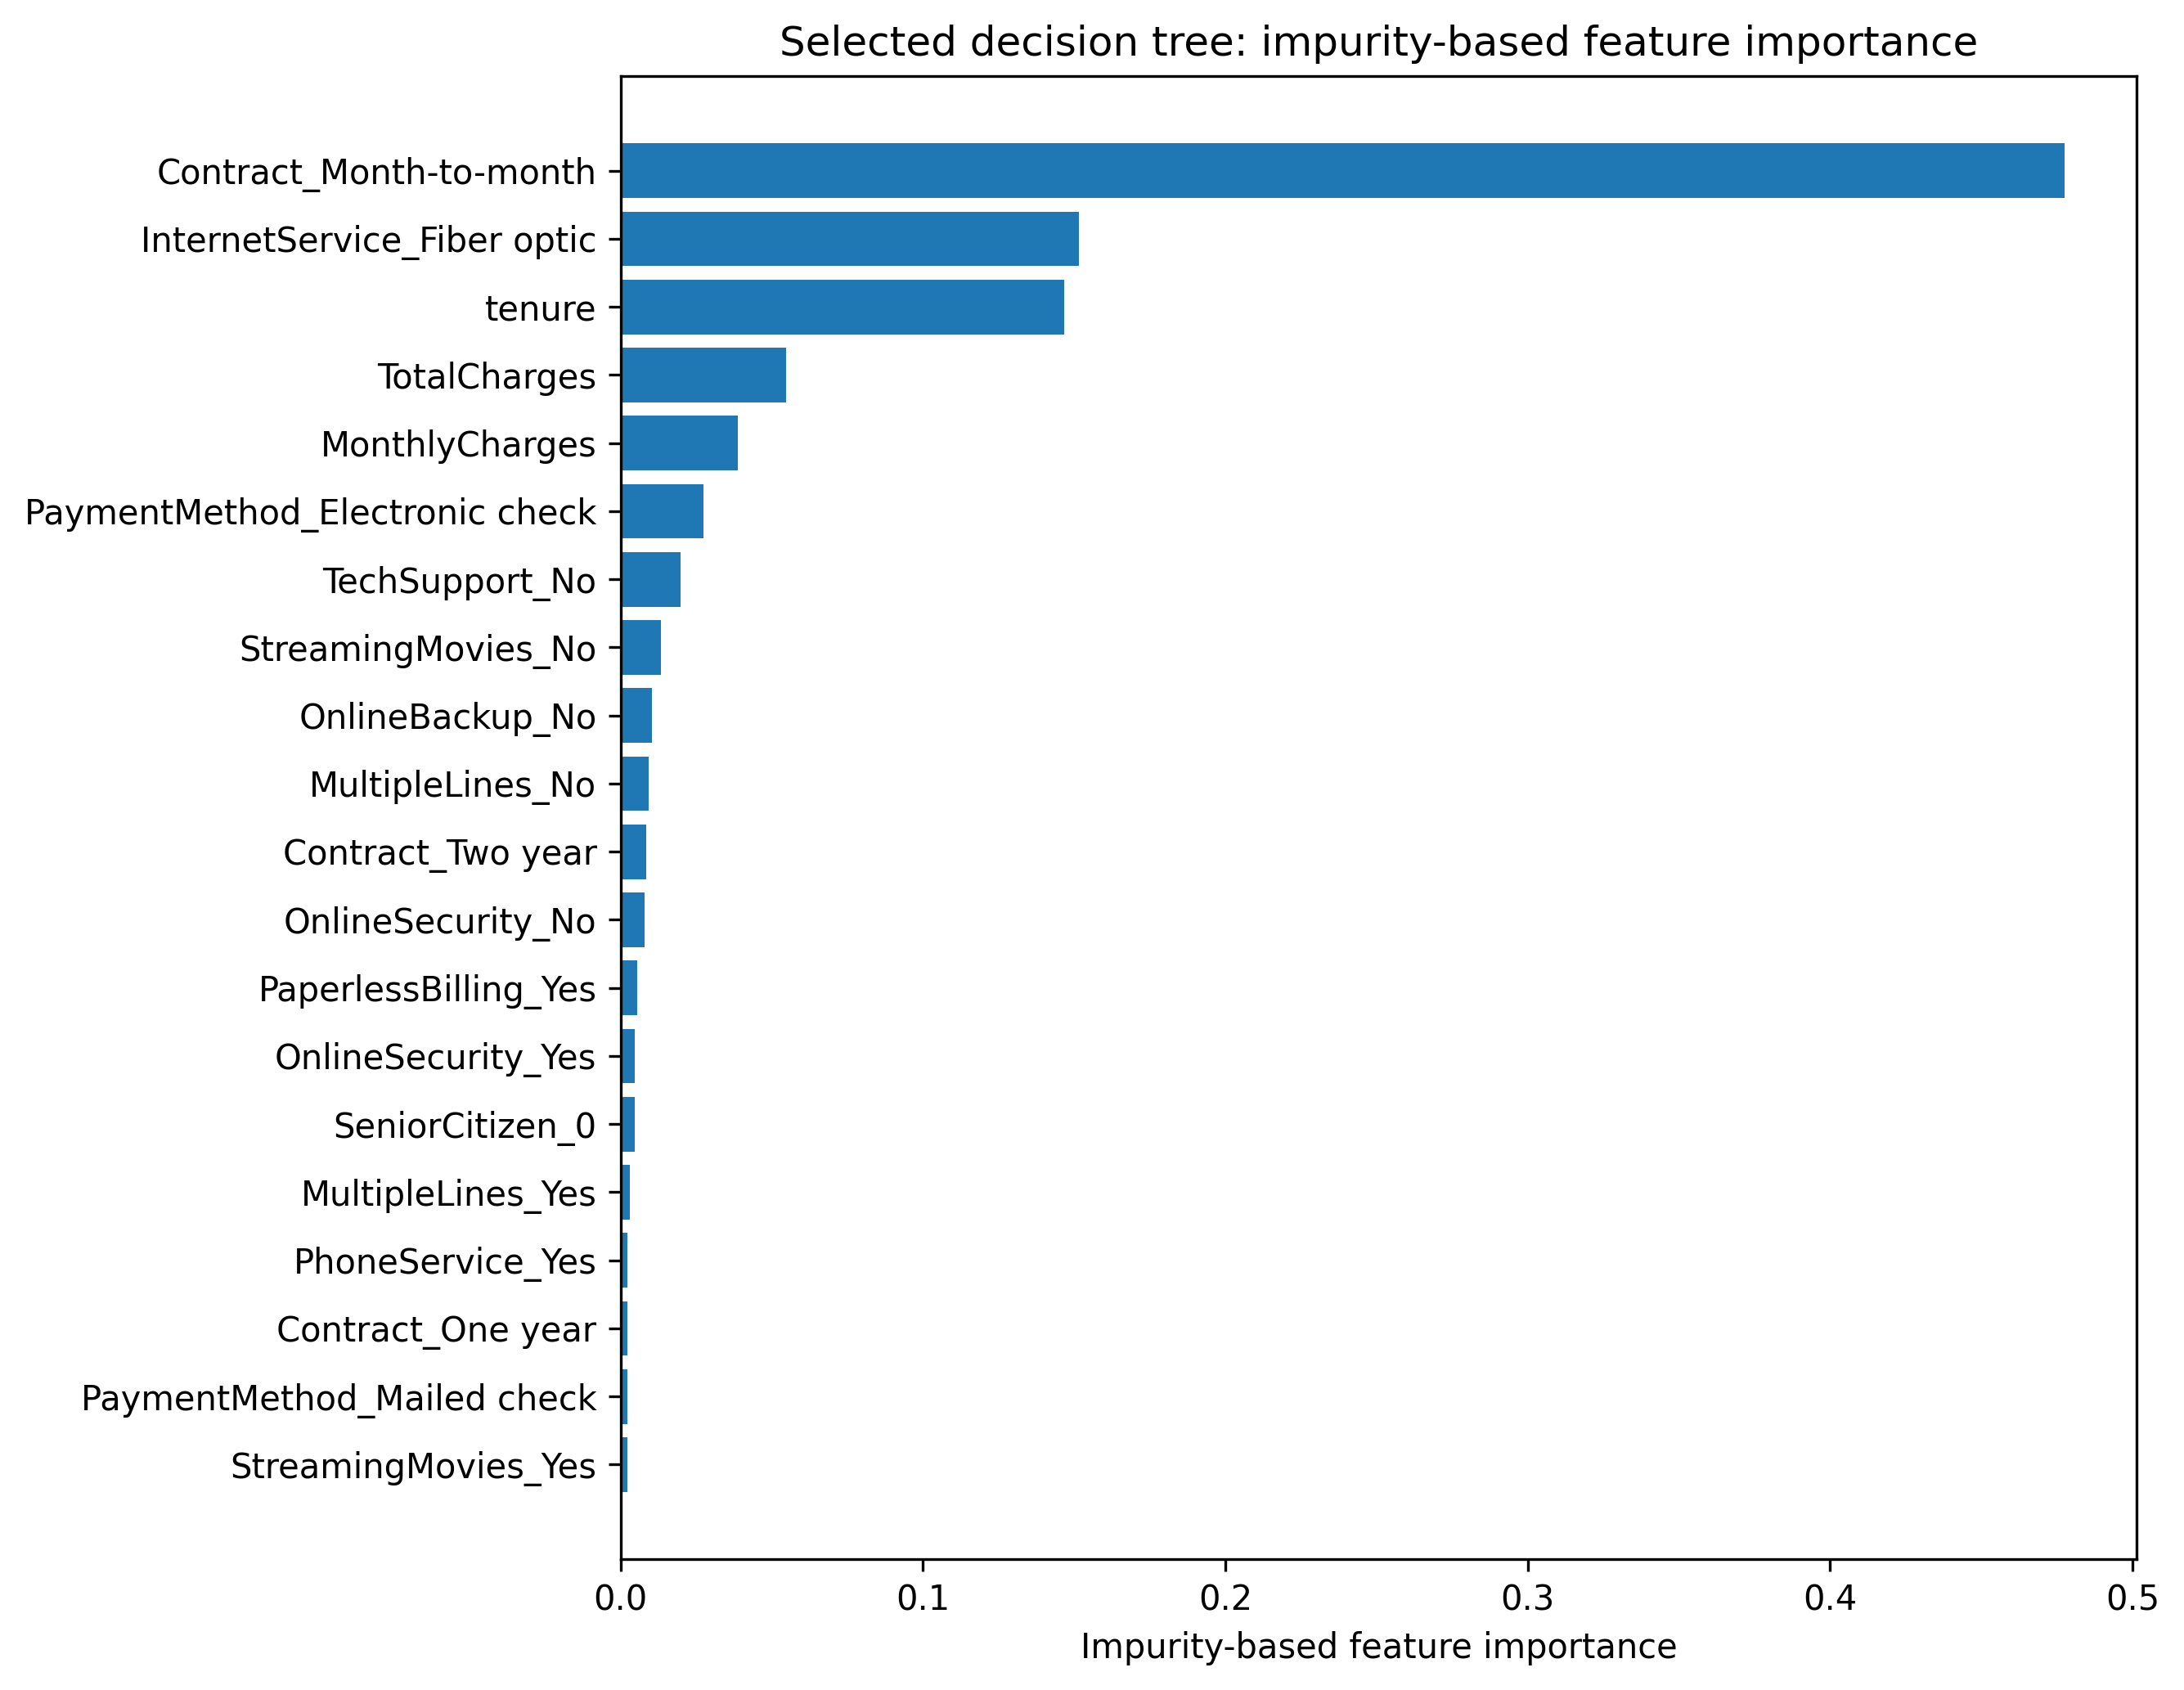
\includegraphics[width=0.82\textwidth]{../figures/decision_tree_feature_importance.png}
\caption{Impurity-based feature importance for the selected decision tree}
\label{fig:decision-tree-feature-importance}
\end{figure}

The feature-importance plot should be interpreted cautiously. Impurity-based importances reflect how much splits reduce impurity inside the fitted tree. They are not causal effects, and they can be influenced by feature cardinality, correlated predictors, and the particular tree structure. Still, they are useful for understanding which variables the selected tree uses most heavily.

\subsection{Summary}

The decision-tree section demonstrates the strengths and weaknesses of single-tree classification. A decision tree provides interpretable rule-based nonlinear classification and naturally captures interactions between features. However, the default unrestricted tree overfits and performs poorly in ranking metrics. Regularization is therefore essential.

The selected single tree is a pre-pruned Gini tree with depth 6, minimum split size 25, and minimum leaf size 10. It reaches development-stage PR-AUC around \(0.628\) and ROC-AUC around \(0.824\). This is a substantial improvement over the default unrestricted tree and a meaningful result for a transparent nonlinear model, but it does not overtake logistic regression in the current development-stage comparison.

This outcome prepares the next modelling stages. Single trees are unstable, but they are the building blocks for bagging, random forests, and boosting. The next tree-based sections can therefore ask whether aggregating many trees improves the variance, ranking quality, and robustness limitations observed here.
